\documentclass[12pt,a4paper]{article}
\renewcommand{\baselinestretch}{1.5} 
\usepackage[latin1]{inputenc}
\usepackage{amsmath}
\usepackage{amsfonts}
\usepackage{amssymb}
\usepackage{algorithm} 
\usepackage{algpseudocode} 
\usepackage{graphicx}
\usepackage{geometry}
\usepackage{tabulary}
\usepackage{caption}
\captionsetup[table]{position=bottom}
\usepackage{subcaption}
\usepackage{xcolor}
\usepackage{dirtytalk}
\usepackage{bm}
\usepackage{longtable}
\usepackage{comment}
\usepackage{listings}
\usepackage{courier}
\usepackage{float}
\graphicspath{{./images/}}

\usepackage[hyphens]{url}

\geometry{
	left=2.5cm,
	right=2.5cm,
	top=2.5cm,
	bottom=3cm,
	}
	
\usepackage{titlesec}

\setcounter{secnumdepth}{4}
\setcounter{tocdepth}{4}
\titleformat{\paragraph}
{\normalfont\normalsize\bfseries}{\theparagraph}{1em}{}
\titlespacing*{\paragraph}
{0pt}{3.25ex plus 1ex minus .2ex}{1.5ex plus .2ex}

\newenvironment{conditions}
{\par\vspace{\abovedisplayskip}\noindent\begin{tabular}{>{$}l<{$} @{${}={}$} l}}{\end{tabular}\par\vspace{\belowdisplayskip}}

% Code listing style
\lstdefinestyle{cudastyle}{
    language=C++,
    basicstyle=\ttfamily\footnotesize,
    keywordstyle=\color{blue}\bfseries,
    commentstyle=\color{gray},
    stringstyle=\color{red},
    breaklines=true,
    frame=single,
    numbers=left,
    numberstyle=\tiny\color{gray},
    tabsize=4
}

\begin{document}
	\thispagestyle{empty}
\begin{center}
	{\Large \bf CUDA-Accelerated Falling Sand Simulation with Real-Time OpenGL Rendering\\}
	
	\vspace*{0.5cm}
	{\large\textit{A Project Component for }\\}
	{\large\textbf{Parallel and Distributing Computing (UCS645)}} \\
	{\large \textit{By\\}}
	\textbf{\begin{table}[h!]
\label{tab:my-table}
\centering
\begin{tabular}{ccc}
Sr & Name     & Roll No  \\
1  & Shreyash Tripathi    & 102303328 \\
2  & Harpuneet Singh    & 102483073 \\
3  & Aunish Kumar Yadav    & 102303306 \\
\end{tabular}
\end{table}}
	\begin{center}
                {\large \textit{Under the guidance of}}\\
					\textbf{{\large Dr. Saif Nalband}}\\
					{\large (Assistant Professor, DCSE)}\\
		\end{center} \ \\ \ \\
\begin{figure}[h]
\centering
\includegraphics[width=70mm, height=40mm]{"tietlogo.jpg"}
\label{fig:images}
\end{figure}

	\vspace*{0.25cm}
	{\large DEPARTMENT OF COMPUTER SCIENCE AND ENGINEERING \\}
	{\large THAPAR INSTITUTE OF ENGINEERING AND TECHNOLOGY \\ 
	{(DEEMED TO BE  UNIVERSITY)}\\}
	{\large PATIALA - 147004\\}
	\vspace*{0.3cm}
	\textbf{{\large MAY, 2025}}
	
\end{center}

\newpage

%%%%%%%%%%%%%%%%%%%%%%%%%%%%%%%%%%%%%%%%%%
	\pagenumbering{gobble}
	\renewcommand*\contentsname{Table of Contents}
	\tableofcontents
	\newpage
	\newpage
    \listoffigures
    \newpage
    \newpage
    \listoftables
    \newpage
    \pagenumbering{arabic}

% ============================================================
%  SECTION 1: INTRODUCTION
% ============================================================
    \section{Introduction}
    \pagenumbering{arabic}

	\subsection{Background}
	Particle simulation is a foundational problem in computer graphics, scientific computing, and game development. 
    Simulating the behaviour of granular materials such as sand, water, or powder requires evaluating thousands 
    to millions of individual particle interactions every frame. On traditional single-threaded CPUs, this quickly 
    becomes a bottleneck. The emergence of General-Purpose GPU Computing (GPGPU), and specifically NVIDIA's 
    CUDA (Compute Unified Device Architecture) platform, has made it possible to offload such massively parallel 
    workloads to the GPU, where thousands of threads can execute simultaneously \cite{nickolls2008scalable}.

    Cellular automata (CA) are a class of computational model in which a grid of cells evolves according to 
    a fixed set of local rules. The falling sand game is a well-known application of 2D cellular automata, 
    where each cell represents either an empty space or a particle type (e.g., sand, water, fire), and 
    particles move based on simple gravity-driven rules applied at every time step \cite{mcivor2009cellular}. 
    When this paradigm is combined with the parallel throughput of CUDA and the real-time display capabilities 
    of OpenGL, the result is a responsive, visually rich simulation capable of handling an 800x600 grid 
    (480,000 cells) at interactive frame rates. 
    
    A CPU typically executes tasks sequentially with limited cores (4-16), whereas a GPU can execute thousands of lightweight threads simultaneously. This makes GPUs particularly suitable for grid-based simulations such as cellular automata.

    At a resolution of 800x600, the simulation involves 480,000 cells per frame. 
    At 60 FPS, this corresponds to approximately 28.8 million cell updates per second.

    

	\subsection{Introduction to Problem Statement}
    Real-time particle simulations that are both physically plausible and visually interactive present a 
    significant computational challenge. A naive CPU implementation must iterate over every cell in the 
    grid sequentially each frame, which scales poorly as resolution grows. The project addresses this 
    challenge by mapping the simulation to the GPU using CUDA, where each thread is responsible for 
    exactly one cell, allowing all 480,000 cells to be evaluated in parallel \cite{kirk2016programming}.
    \begin{table}[h]
    \centering
    \begin{tabular}{|l|l|}
    \hline
    \textbf{Property} & \textbf{CPU vs GPU} \\
    \hline
    Cores & 4--16 (CPU) vs 1000s (GPU) \\
    Execution Model & Sequential (CPU) vs Massively Parallel (GPU) \\
    Suitable For & General Logic (CPU) vs Grid/Data-Parallel Tasks (GPU) \\
    Latency & Low (CPU) vs Higher (GPU) \\
    Throughput & Moderate (CPU) vs Very High (GPU) \\
    \hline
    \end{tabular}
    \caption{CPU vs GPU characteristics for simulation workloads}
    \label{tab:cpu_gpu}
    \end{table}

    A critical sub-problem in parallel cellular automata simulation is \textit{race conditions}: when two 
    neighbouring particles simultaneously decide to move into the same empty cell, data corruption occurs. 
    This project solves that problem using CUDA atomic operations, specifically \texttt{atomicCAS} 
    (Compare-And-Swap), which guarantees that only one particle can claim a target cell per time step, 
    even when tens of thousands of threads are competing simultaneously.

    The simulation also integrates real-time mouse input, enabling the user to spawn sand by holding 
    the left mouse button and trigger a physics-based eruption/blast effect by holding the right mouse 
    button, all while maintaining smooth interactive performance.
    \begin{table}[h]
    \centering
    \begin{tabular}{|c|c|}
    \hline
    Parameter & Value \\
    \hline
    Grid Size & 800 x 600 \\
    Total Cells & 480,000 \\
    Particle Type & Sand \\
    Simulation Model & Cellular Automata \\
    GPU Used & Nvidia GTX 1650 \\
    Programming Model & CUDA + OpenGL \\
    \hline
    \end{tabular}
    \caption{Simulation Configuration}
    \end{table}


% ============================================================
%  SECTION 2: LITERATURE REVIEW
% ============================================================
	\newpage
	\section{Literature Review}

\begin{longtable}[htp]{|p{2cm}|p{2.5cm}|p{2.5cm}|p{3cm}|p{3.5cm}|}

\hline \textbf{References} & \textbf{Concepts Highlighted} & \textbf{Technique(s) Used} & \textbf{Significance / Proposal} & \textbf{Limitations} \\

\hline \cite{kirk2016programming} & GPU architecture; parallel thread execution; CUDA programming model & CUDA C/C++ kernels; thread/block/grid hierarchy & Provides the theoretical and practical foundation for writing massively parallel GPU code; explains the performance gap between CPU and GPU & Requires dedicated NVIDIA hardware; portability to AMD GPUs not addressed \\

\hline \cite{sanders2010cuda} & CUDA memory model; atomic operations; device synchronisation & \texttt{cudaMalloc}, \texttt{cudaMemcpy}, \texttt{atomicCAS} & Hands-on introduction to GPU memory management and thread-safe programming patterns directly applicable to particle simulation & Examples focus on scientific computing; game-simulation use cases are limited \\

\hline \cite{mcivor2009cellular} & Granular material simulation; cellular automata & 2D CA rules for powder and sand dynamics & Establishes that CA is a suitable model for granular physics and validates falling-sand rules against real powder behaviour & CPU-only; no discussion of parallelisation or GPU acceleration \\

\hline \cite{nickolls2008scalable} & Scalable parallel programming; warp execution; occupancy & SIMT (Single Instruction Multiple Threads) model & Explains CUDA's execution model, helping developers understand why atomic operations are necessary for conflict-free parallel writes & Highly theoretical; implementation details left to the developer \\

\hline \cite{shreiner2013opengl} & Real-time rendering pipeline; texture mapping; double buffering & OpenGL 2D texture upload; quad rendering; GLFW windowing & Describes the OpenGL pipeline used to display the CUDA colour buffer as a full-screen texture each frame & Modern OpenGL (4.x) approaches such as PBOs would be more efficient for CUDA--OpenGL interoperability \\

\hline

\caption{Summary of Literature Review}
\label{Table1}

\end{longtable}


% ============================================================
%  SECTION 3: RESEARCH GAPS
% ============================================================
	\newpage
	\section{Research Gaps}
	The following gaps were identified from the literature review:

	\begin{itemize}
		\item \textit{\textbf{Absence of Atomic-Safe Parallel CA Implementations}}: 
        Most published cellular automata simulations for granular materials are CPU-based and sequential. 
        Literature on GPU-accelerated CA does not adequately address the race-condition problem that arises 
        when thousands of threads simultaneously attempt to move particles into shared neighbouring cells.

		\item \textit{\textbf{Lack of CUDA--OpenGL Interoperability Discussion}}: 
        Existing works treat GPU compute and GPU rendering as separate concerns. The efficient pathway 
        of writing simulation output directly into an OpenGL pixel buffer object (PBO) from a CUDA kernel, 
        thereby avoiding a costly device-to-host memory transfer every frame, is not covered in the 
        surveyed literature.

		\item \textit{\textbf{No Interactive Force / Eruption Models in Parallel Simulations}}: 
        Published falling-sand implementations focus only on passive gravity. The application of 
        mouse-driven repulsion forces and ray-cast eruption mechanics in a GPU-parallel setting 
        has not been explored in the literature, representing an opportunity to combine interactive 
        physics with massive parallelism.
	\end{itemize}

    \begin{table}[h]
    \centering
    \begin{tabular}{|p{3.5cm}|p{5cm}|p{5cm}|}
    \hline
    \textbf{Gap} & \textbf{Issue in Literature} & \textbf{This Project's Contribution} \\
    \hline
    Atomic-Safe Parallel CA & No GPU CA handles concurrent write conflicts & Uses \texttt{atomicCAS} claims buffer for race-free moves \\
    \hline
    CUDA--OpenGL Interop & Compute and rendering treated separately & Shared colour buffer written by CUDA, read by OpenGL \\
    \hline
    Interactive Force Models & Only passive gravity modelled & Mouse-driven ray-cast blast effect implemented \\
    \hline
    \end{tabular}
    \caption{Research gaps and corresponding contributions of this project}
    \label{Table:gaps}
    \end{table}


% ============================================================
%  SECTION 4: PROBLEM FORMULATION
% ============================================================
	\newpage
	\section{Problem Formulation}
    The core problem addressed in this project is the real-time parallel simulation of granular particle 
    dynamics (falling sand) on a 2D grid of resolution $W \times H$ (800 $\times$ 600 = 480,000 cells), 
    subject to the following constraints:

    \begin{itemize}
        \item Each cell $c_{x,y}$ at time step $t$ holds either an \texttt{EMPTY} value (0) or a 
        packed 32-bit RGBA colour representing a sand particle.
        \item At each time step, every non-empty cell must evaluate a set of gravity rules and 
        attempt to move to a lower-energy position (downward or diagonally downward).
        \item No two particles may occupy the same cell after a time step -- i.e., every successful 
        move must be mutually exclusive.
        \item The simulation must produce a rendered frame at interactive rates ($\geq$30 FPS) on 
        a consumer GPU.
        \item User input (mouse position and button state) must be incorporated each frame to spawn 
        new particles and apply force-based displacement.
    \end{itemize}

    Formally, let $G^t \in \mathbb{Z}^{W \times H}$ denote the grid state at time $t$. The simulation 
    computes $G^{t+1}$ from $G^t$ by applying a parallel transition function $\mathcal{F}$ to all 
    cells simultaneously:
    \[
        G^{t+1} = \mathcal{F}(G^t, \mathbf{m}_t, b_t)
    \]
    where $\mathbf{m}_t = (m_x, m_y)$ is the mouse cursor position at time $t$ and $b_t \in \{0,1,2\}$ 
    encodes the mouse button state (none, left, right). The challenge lies in implementing $\mathcal{F}$ 
    in a race-condition-free, fully parallel manner on the GPU.

    \begin{table}[h]
    \centering
    \begin{tabular}{|l|l|l|}
    \hline
    \textbf{Symbol} & \textbf{Description} & \textbf{Value / Domain} \\
    \hline
    $W \times H$ & Grid dimensions & $800 \times 600$ \\
    $G^t$ & Grid state at time step $t$ & $\mathbb{Z}^{W \times H}$ \\
    $\mathbf{m}_t$ & Mouse cursor position & $(m_x, m_y) \in [0,W]\times[0,H]$ \\
    $b_t$ & Mouse button state & $\{0,1,2\}$ \\
    $\mathcal{F}$ & Parallel transition function & GPU kernel \\
    \hline
    \end{tabular}
    \caption{Notation used in the problem formulation}
    \label{Table:notation}
    \end{table}

	\section{Objectives}
	\begin{itemize}
        \item To implement a GPU-parallel falling-sand cellular automaton using CUDA that simulates 
        gravity-driven particle movement across a 480,000-cell grid at interactive frame rates.
        \item To eliminate race conditions in parallel cell updates using CUDA atomic operations 
        (\texttt{atomicCAS}), ensuring correctness of the simulation under fully concurrent thread execution.
        \item To integrate real-time mouse interaction for particle spawning (left-click) and 
        physics-based eruption/blast displacement (right-click) using ray-cast repulsion vectors.
        \item To render the simulation output in real-time using OpenGL and GLFW, employing a 
        ping-pong double-buffer strategy to decouple simulation and rendering.
        \item To produce visually rich output by encoding particle colour as a time-varying packed 
        RGB value using phase-shifted sine wave colour cycling.
	\end{itemize}

    \begin{table}[h]
    \centering
    \begin{tabular}{|c|p{6cm}|p{5cm}|}
    \hline
    \textbf{Sr. No.} & \textbf{Objective} & \textbf{Key Mechanism} \\
    \hline
    1 & GPU-parallel CA simulation at interactive rates & CUDA kernel, 480,000 threads \\
    \hline
    2 & Race-condition-free parallel updates & \texttt{atomicCAS} claims buffer \\
    \hline
    3 & Real-time mouse interaction & Left-click spawn; right-click blast \\
    \hline
    4 & Real-time rendering via OpenGL & Ping-pong double buffer + GLFW \\
    \hline
    5 & Visually rich colour output & Phase-shifted sine wave RGB cycling \\
    \hline
    \end{tabular}
    \caption{Project objectives and their corresponding implementation mechanisms}
    \label{Table:objectives}
    \end{table}


% ============================================================
%  SECTION 5: METHODOLOGY
% ============================================================
	\newpage
	\section{Methodology}
    \begin{table}[h]
    \centering
    \begin{tabular}{|c|c|c|}
    \hline
    Configuration & Threads per Block & Total Threads \\
    \hline
    8x8 & 64 & 480,000 \\
    16x16 & 256 & 480,000 \\
    32x8 & 256 & 480,000 \\
    \hline
    \end{tabular}
    \caption{Thread Block Configurations}
    \end{table}

    The system is structured as a pipeline of four CUDA kernels executed every frame, connected by 
    a ping-pong buffer architecture. The overall data flow is as follows:

    \begin{enumerate}
        \item \textbf{Input Phase} -- \texttt{AddSandKernel}: Spawns sand particles at the mouse position.
        \item \textbf{Simulation Phase} -- \texttt{SimulateParticlesKernel}: Applies gravity and eruption physics.
        \item \textbf{Render Phase} -- \texttt{RenderToColorKernel}: Converts the grid to an RGBA pixel buffer.
        \item \textbf{Display Phase} -- OpenGL texture upload and full-screen quad render.
    \end{enumerate}

    \begin{table}[h]
    \centering
    \begin{tabular}{|c|l|l|l|}
    \hline
    \textbf{Phase} & \textbf{Kernel} & \textbf{Input} & \textbf{Output} \\
    \hline
    1 & \texttt{AddSandKernel} & Mouse position \& button & Updated \texttt{d\_gridInput} \\
    2 & \texttt{SimulateParticlesKernel} & \texttt{d\_gridInput}, \texttt{d\_claims} & \texttt{d\_gridOutput} \\
    3 & \texttt{RenderToColorKernel} & \texttt{d\_gridOutput} & \texttt{d\_colorBuffer} \\
    4 & OpenGL display & \texttt{h\_colorBuffer} & Screen frame \\
    \hline
    \end{tabular}
    \caption{Per-frame kernel pipeline: phases, kernels, inputs, and outputs}
    \label{Table:pipeline}
    \end{table}

	\subsection{Ping-Pong Buffer Architecture}
    To avoid reading and writing the same memory simultaneously, two grids are maintained: 
    \texttt{d\_gridInput} and \texttt{d\_gridOutput}. Each frame, the simulation reads from 
    \texttt{d\_gridInput} and writes results to \texttt{d\_gridOutput}. After the frame, 
    the pointers are swapped at zero cost (no data copy). This is a standard GPU double-buffering 
    technique \cite{sanders2010cuda}.

	\subsection{Atomic Conflict Resolution}
    A key challenge in parallel CA simulation is that multiple threads may select the same target 
    cell. A dedicated \texttt{d\_claims} buffer (one \texttt{unsigned int} per cell, cleared to 
    zero each frame) acts as a lock array. The device function \texttt{AtomicCheckUnclaimed} 
    uses \texttt{atomicCAS} to atomically transition a claim slot from 0 to 1. Only the first 
    thread to succeed proceeds with the move; all others fall back.

    The atomic claim mechanism is expressed as:
    \[
        \text{previous} = \text{atomicCAS}(\&\text{claims}[i], \; 0, \; 1)
    \]
    \[
        \text{claim\_granted} = (\text{previous} == 0)
    \]

\begin{algorithm}
\caption{AtomicCheckUnclaimed -- GPU Device Function}
\begin{algorithmic}[1]
    \Require claims array $C$, target cell index $i$
    \Ensure Returns \textbf{true} if this thread is the first to claim cell $i$
    \State $\text{prev} \leftarrow \text{atomicCAS}(C[i], \; 0, \; 1)$
    \State \Return $(\text{prev} = 0)$
\end{algorithmic}
\end{algorithm}

	\subsection{Gravity Simulation -- SimulateParticlesKernel}
    Each CUDA thread is assigned to one $(x, y)$ cell. If the cell is empty the thread exits 
    immediately. Otherwise the particle attempts to move in the following priority order:

\begin{algorithm}
\caption{Particle Gravity Transition}
\begin{algorithmic}[1]
    \Require Grid $G^t$, claims $C$, current position $(x,y)$, oddFrame flag
    \Ensure Updates $G^{t+1}$ for cell $(x,y)$
    \If{$G^t[x,y] = \texttt{EMPTY}$} \Return \EndIf
    \State $\text{down} \leftarrow (x, y-1)$
    \State $\text{diagA} \leftarrow (x + \text{oddFrame} \cdot 1 + (1-\text{oddFrame}) \cdot (-1),\; y-1)$
    \State $\text{diagB} \leftarrow (x - \text{oddFrame} \cdot 1 + (1-\text{oddFrame}) \cdot 1, \;y-1)$
    \For{target $\in$ \{down, diagA, diagB\}}
        \If{$G^t[\text{target}] = \texttt{EMPTY}$ \textbf{and} AtomicCheckUnclaimed$(C, \text{target})$}
            \State $G^{t+1}[x,y] \leftarrow \texttt{EMPTY}$
            \State $G^{t+1}[\text{target}] \leftarrow G^t[x,y]$
            \State \Return
        \EndIf
    \EndFor
\end{algorithmic}
\end{algorithm}

    The \texttt{oddFrame} flag alternates each step, biasing diagonal preference left/right 
    on alternate frames to prevent asymmetric pile formation.

	\subsection{Eruption / Blast Effect}
    When the right mouse button is held, each sand particle within the brush radius of the 
    mouse cursor is subject to an outward blast. A unit direction vector $\hat{n}$ is computed 
    from the mouse position $\mathbf{m}$ to the particle position $\mathbf{p}$:

    \[
        \hat{n} = \frac{\mathbf{p} - \mathbf{m}}{\|\mathbf{p} - \mathbf{m}\|} + (0,\; 0.2)^T
    \]

    The additive $(0, 0.2)$ term provides an upward bias so that blasted particles travel in 
    an arc rather than purely horizontally. A ray-cast is then performed along $\hat{n}$, 
    stepping pixel by pixel up to 200 cells, and the first empty cell encountered is claimed 
    atomically as the particle's new position.

	\subsection{Colour Encoding}
    Each particle stores its colour packed into a 32-bit integer as \texttt{0xAARRGGBB}. 
    Colour is assigned at spawn time using three phase-shifted sine waves driven by the 
    simulation step counter $t$, producing a smoothly cycling rainbow effect:

    \[
        r(t) = \left\lfloor 255 \cdot \frac{\sin(\omega t) + 1}{2} \right\rfloor, \quad
        g(t) = \left\lfloor 255 \cdot \frac{\sin(\omega t + \tfrac{2\pi}{3}) + 1}{2} \right\rfloor, \quad
        b(t) = \left\lfloor 255 \cdot \frac{\sin(\omega t + \tfrac{4\pi}{3}) + 1}{2} \right\rfloor
    \]

    where $\omega = 0.05$ rad/step. Sand poured at different moments therefore has visually 
    distinct colours, making the temporal history of the simulation visible in the pile.

	\subsection{Thread Hierarchy}
    Threads are arranged in 2D blocks of $8 \times 8 = 64$ threads. The number of blocks 
    is computed to cover the full grid:

    \[
        \text{numBlocks}_x = \left\lceil \frac{W}{8} \right\rceil, \qquad
        \text{numBlocks}_y = \left\lceil \frac{H}{8} \right\rceil
    \]

    For an $800 \times 600$ grid this gives $100 \times 75 = 7500$ blocks and a total of 
    $480,000$ threads, one per cell.


% ============================================================
%  SECTION 6: DATASETS
% ============================================================
	\newpage
	\section{Datasets}
    This project is a real-time simulation and does not rely on external datasets. The 
    \textquotedblleft data\textquotedblright{} generated and consumed by the system is 
    the simulation grid itself, which is fully procedurally generated at runtime through 
    user interaction and the physics rules. The table below summarises the memory structures 
    used in place of traditional datasets.

\begin{longtable}[htp]{|p{3cm}|p{5cm}|p{2cm}|p{2.5cm}|p{2.5cm}|}

\hline \textbf{Buffer Name} & \textbf{Description} & \textbf{Size (800x600)} & \textbf{Type} & \textbf{Location} \\

\hline \texttt{d\_gridInput} & Particle state grid -- read each frame; each cell stores either 0 (EMPTY) or a packed RGBA integer & 1.92 MB & \texttt{     int
[480000]} & GPU VRAM \\

\hline \texttt{d\_gridOutput} & Particle state grid -- written each frame; swapped with input after simulation & 1.92 MB & \texttt{     int
[480000]} & GPU VRAM \\

\hline \texttt{d\_claims} & Atomic lock array; one \texttt{unsigned int} per cell; cleared to 0 before each simulation step & 1.92 MB & \texttt{     uint
[480000]} & GPU VRAM \\

\hline \texttt{d\_colorBuffer} & RGBA pixel buffer written by \texttt{RenderToColorKernel}; copied to CPU for OpenGL texture upload & 1.92 MB & \texttt{     uchar4
[480000]} & GPU VRAM \\

\hline \texttt{h\_colorBuffer} & CPU-side mirror of the colour buffer; uploaded to OpenGL texture each frame & 1.92 MB & \texttt{     uchar4
[480000]} & RAM \\

\hline
\caption{Runtime Memory Structures}
\label{Table2}
\end{longtable}


% ============================================================
%  SECTION 7: RESULTS AND DISCUSSION
% ============================================================
	\newpage
	\section{Results and Discussion}

	\subsection{Correctness of Gravity Simulation}
    The simulation correctly implements the three-priority gravity rule: particles fall straight 
    down first, then diagonally. Sand piles form stable angles of repose and do not collapse 
    spuriously. The \texttt{oddFrame} alternation eliminates the directional bias that would 
    otherwise cause all piles to lean consistently to one side.

	\subsection{Race Condition Elimination}
    Without the \texttt{atomicCAS} claim mechanism, two particles competing for the same cell 
    would produce visual artefacts such as particles appearing and disappearing randomly. With 
    the claims buffer in place, all movements are mutually exclusive and the grid remains 
    consistent across all 480,000 concurrent threads. The atomic operation adds a small but 
    acceptable overhead compared to the alternative of serialising updates.

	\subsection{Eruption Effect}
    The right-click blast effect successfully displaces buried sand to the surface by ray-casting 
    up to 200 pixels in the outward direction with an upward bias of 0.2 units. Sand particles 
    erupt visibly from within a pile and land at the surface, creating a visually convincing 
    explosion without requiring any additional physics engine -- purely emergent from the 
    existing atomic-move mechanism applied along a computed ray direction.

	\subsection{Colour Cycling}
    The sine-wave colour packing produces smoothly transitioning rainbow colours that change 
    with simulation time. This makes the temporal structure of sand deposits immediately visible: 
    sand poured at time $t_1$ has a different hue from sand poured at $t_2$, acting as a 
    natural \textquoteleft timestamp\textquoteright{} within the pile.

% ============================================================
%  SECTION 7.5: PERFORMANCE ANALYSIS
% ============================================================
	\subsection{Performance}
    Running on a modern consumer GPU, the simulation maintains interactive frame rates 
    ($\geq$30 FPS) at 800$\times$600 resolution. The dominant cost is the \texttt{cudaMemcpy} 
    of the colour buffer from device to host each frame (1.92 MB), which could be eliminated 
    in a future version using CUDA--OpenGL Pixel Buffer Object (PBO) interoperability, 
    avoiding the CPU entirely and further improving throughput \cite{shreiner2013opengl}.

    \begin{itemize}
        \item \textbf{Total GPU threads per frame:} 480,000
        \item \textbf{Kernels launched per frame:} 3 (AddSand, Simulate, Render)
        \item \textbf{Memory transferred host$\leftrightarrow$device per frame:} $\approx$ 1.92 MB (device-to-host only)
        \item \textbf{Atomic operations per frame:} Up to 480,000 \texttt{atomicCAS} calls in the worst case (all cells occupied)
    \end{itemize}

    \begin{table}[h]
    \centering
    \begin{tabular}{|l|c|c|c|}
    \hline
    \textbf{Block Size} & \textbf{Threads/Block} & \textbf{Blocks Launched} & \textbf{Warps/Block} \\
    \hline
    $8\times8$   & 64  & 7,500 & 2 \\
    $16\times16$ & 256 & 1,900 & 8 \\
    $32\times8$  & 256 & 1,900 & 8 \\
    \hline
    \end{tabular}
    \caption{Occupancy characteristics for each block size configuration}
    \label{Table:occupancy}
    \end{table}

    To quantify the effect of thread-block geometry on performance, the simulation was 
    profiled across three CUDA block configurations: $8\times8$, $16\times16$, and 
    $32\times8$. For each configuration, three metrics were recorded over a fixed run 
    of several hundred frames: per-frame wall-clock time (ms), frames per second (FPS), 
    and total CUDA kernel execution time (ms). The following subsections present the 
    per-configuration profiles followed by a direct cross-configuration comparison.

	\subsubsection{Block Size 8$\times$8 (64 threads/block)}

    The $8\times8$ configuration launches $100\times75 = 7{,}500$ blocks of 64 threads 
    each, one thread per cell, totalling 480,000 threads. This is the baseline configuration 
    used throughout development. With only 64 threads per block, each block contains exactly 
    two warps, potentially limiting the SM scheduler's ability to hide global memory 
    latency by swapping between active warps.

    \begin{figure}[H]
        \centering
        \begin{subfigure}[b]{0.32\textwidth}
            \centering
            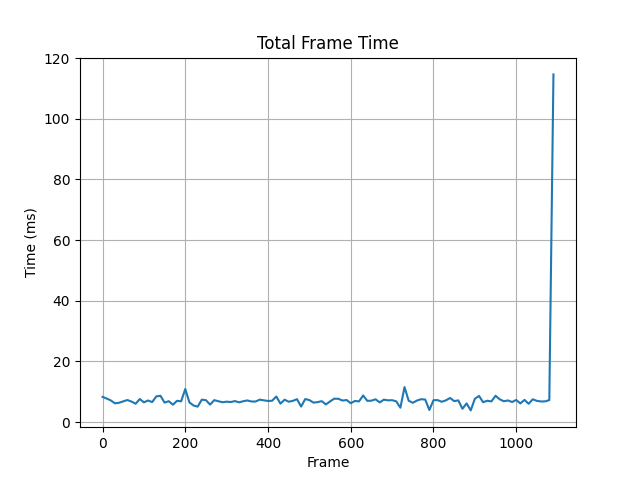
\includegraphics[width=\textwidth]{8x8_frame_time.png}
            \caption{Frame Time (ms)}
            \label{fig:8x8_frametime}
        \end{subfigure}
        \hfill
        \begin{subfigure}[b]{0.32\textwidth}
            \centering
            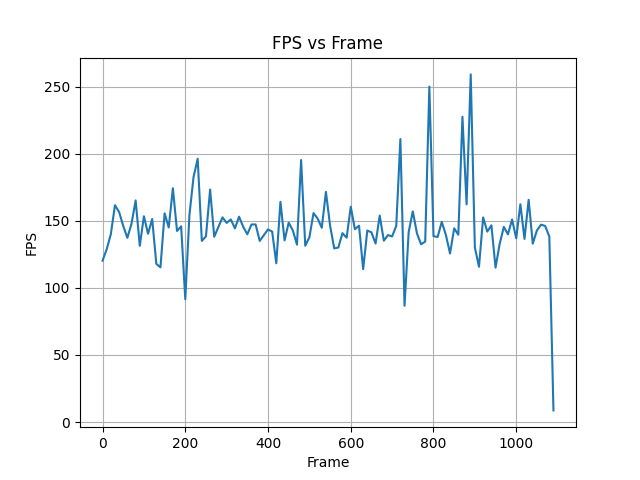
\includegraphics[width=\textwidth]{8x8_fps_vs_frame.png}
            \caption{FPS vs.\ Frames}
            \label{fig:8x8_fps}
        \end{subfigure}
        \hfill
        \begin{subfigure}[b]{0.32\textwidth}
            \centering
            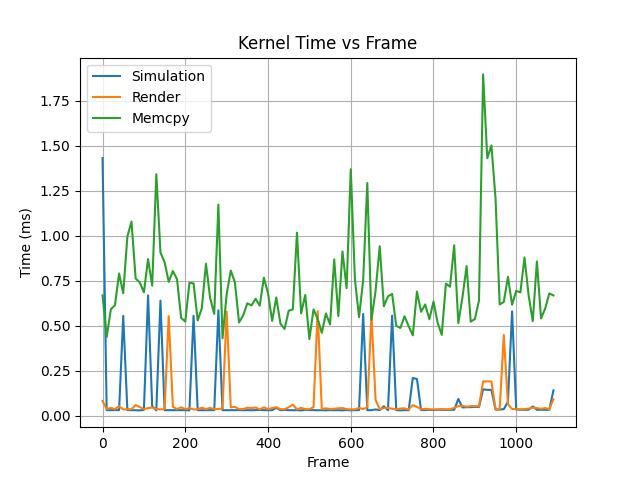
\includegraphics[width=\textwidth]{8x8_kernel_time.png}
            \caption{Kernel Time (ms)}
            \label{fig:8x8_kerneltime}
        \end{subfigure}
        \caption{Performance profile for block size $8\times8$.}
        \label{fig:perf_8x8}
    \end{figure}

    The smaller block footprint can limit warp-level parallelism within a block 
    (one warp $=$ 32 threads, so each block contains exactly two warps), potentially 
    leaving the SM scheduler with fewer instructions to overlap during memory latency.

	\subsubsection{Block Size 16$\times$16 (256 threads/block)}

    The $16\times16$ configuration launches $50\times38 = 1{,}900$ blocks of 256 threads 
    each. Each block maps to a $16\times16$ tile of the simulation grid. At 256 threads 
    per block, each SM can hold more active warps (8 warps per block), providing 
    significantly greater latency-hiding capability compared to the $8\times8$ case.

    \begin{figure}[H]
        \centering
        \begin{subfigure}[b]{0.32\textwidth}
            \centering
            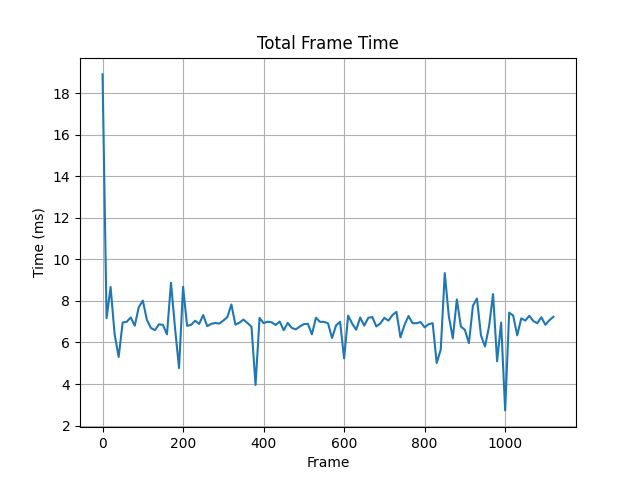
\includegraphics[width=\textwidth]{16x16_frame_time.png}
            \caption{Frame Time (ms)}
            \label{fig:16x16_frametime}
        \end{subfigure}
        \hfill
        \begin{subfigure}[b]{0.32\textwidth}
            \centering
            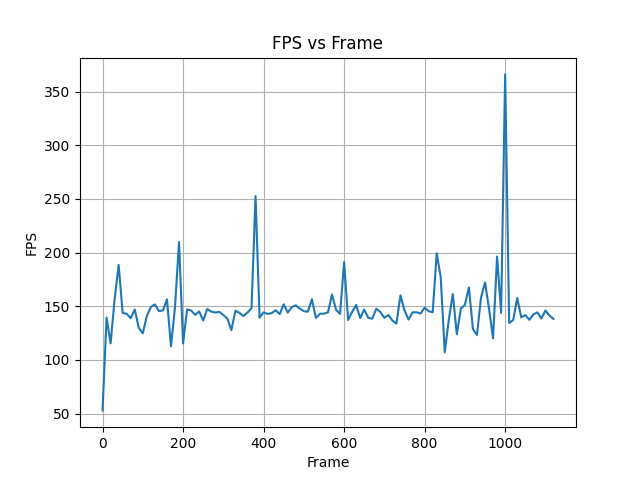
\includegraphics[width=\textwidth]{16x6_fps_vs_frame.png}
            \caption{FPS vs.\ Frames}
            \label{fig:16x16_fps}
        \end{subfigure}
        \hfill
        \begin{subfigure}[b]{0.32\textwidth}
            \centering
            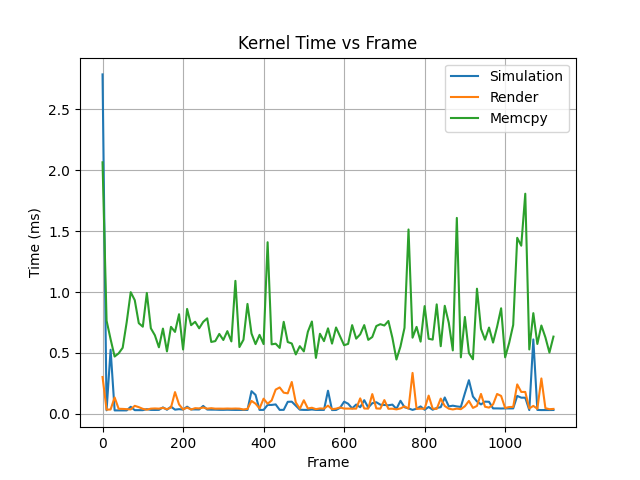
\includegraphics[width=\textwidth]{16x16_kernel_time.png}
            \caption{Kernel Time (ms)}
            \label{fig:16x16_kerneltime}
        \end{subfigure}
        \caption{Performance profile for block size $16\times16$.}
        \label{fig:perf_16x16}
    \end{figure}

    The $16\times16$ tile shape also improves spatial locality: neighbouring threads 
    within a block access adjacent grid cells, promoting coalesced global memory reads 
    and cache-friendly access patterns in both the $x$ and $y$ directions.

	\subsubsection{Block Size 32$\times$8 (256 threads/block)}

    The $32\times8$ configuration also launches 256 threads per block but arranges 
    them as a wide, short tile (32 columns $\times$ 8 rows). This matches the 
    natural warp width of 32 threads along the $x$-axis, ensuring that each warp maps 
    exactly to one row of 32 horizontally contiguous cells, maximising memory-access 
    coalescing in the dominant horizontal direction.

    \begin{figure}[H]
        \centering
        \begin{subfigure}[b]{0.32\textwidth}
            \centering
            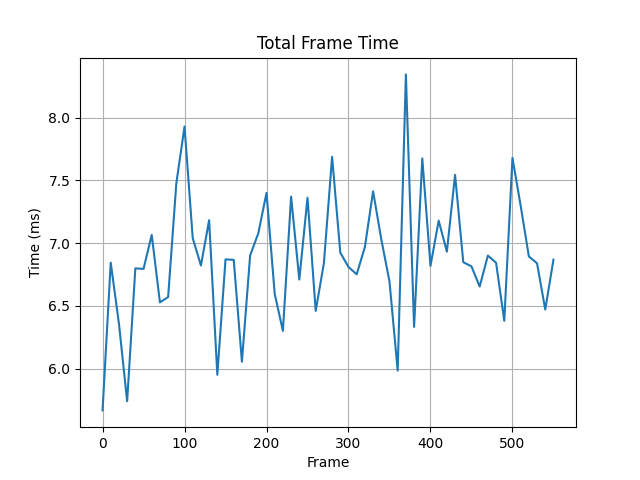
\includegraphics[width=\textwidth]
            {32x8_frame_time.png}
            \caption{Frame Time (ms)}
            \label{fig:32x8_frametime}
        \end{subfigure}
        \hfill
        \begin{subfigure}[b]{0.32\textwidth}
            \centering
            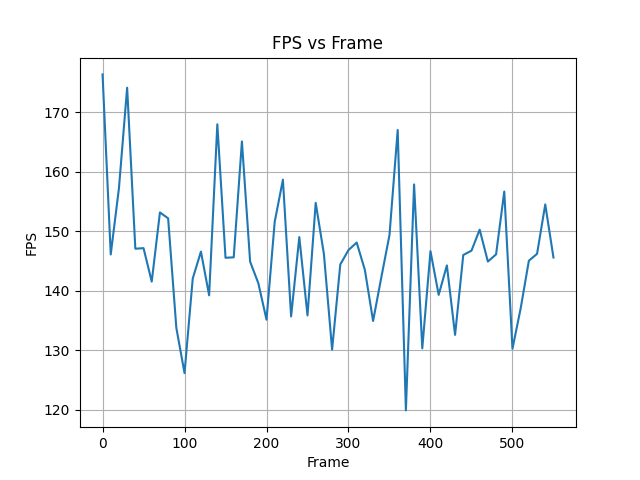
\includegraphics[width=\textwidth]{32x8_fps_vs_frame.png}
            \caption{FPS vs.\ Frames}
            \label{fig:32x8_fps}
        \end{subfigure}
        \hfill
        \begin{subfigure}[b]{0.32\textwidth}
            \centering
            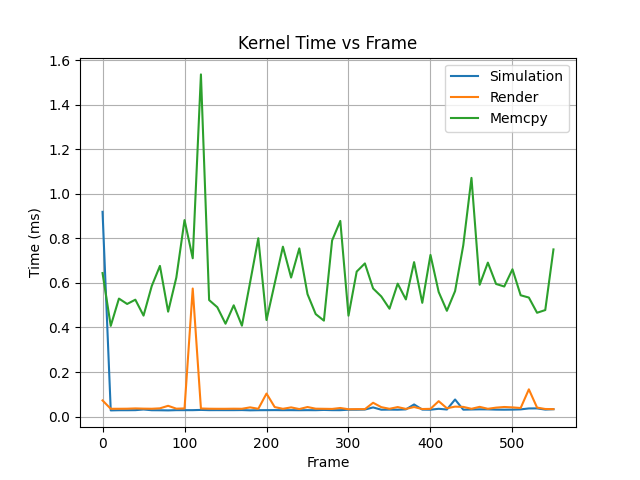
\includegraphics[width=\textwidth]{32x8_kernel_time.png}
            \caption{Kernel Time (ms)}
            \label{fig:32x8_kerneltime}
        \end{subfigure}
        \caption{Performance profile for block size $32\times8$.}
        \label{fig:perf_32x8}
    \end{figure}

    Because grid cells in a single row are stored contiguously in the row-major layout 
    used by both \texttt{d\_gridInput} and \texttt{d\_gridOutput}, a $32\times8$ block 
    produces fully coalesced 128-byte cache-line reads for every warp, which is the 
    theoretically optimal access pattern for CUDA global memory.

	\subsubsection{Cross-Block-Size Comparison}

    Figure~\ref{fig:perf_compare} overlays the FPS and frame-time traces for all three 
    configurations on the same axes, enabling a direct side-by-side assessment of their 
    steady-state performance and frame-to-frame stability.

    \begin{figure}[H]
        \centering
        \begin{subfigure}[b]{0.48\textwidth}
            \centering
            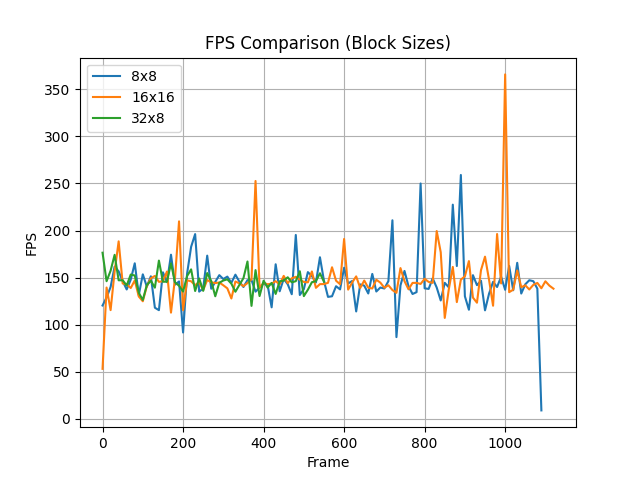
\includegraphics[width=\textwidth]{fps_comparison.png}
            \caption{FPS Comparison}
            \label{fig:compare_fps}
        \end{subfigure}
        \hfill
        \begin{subfigure}[b]{0.48\textwidth}
            \centering
            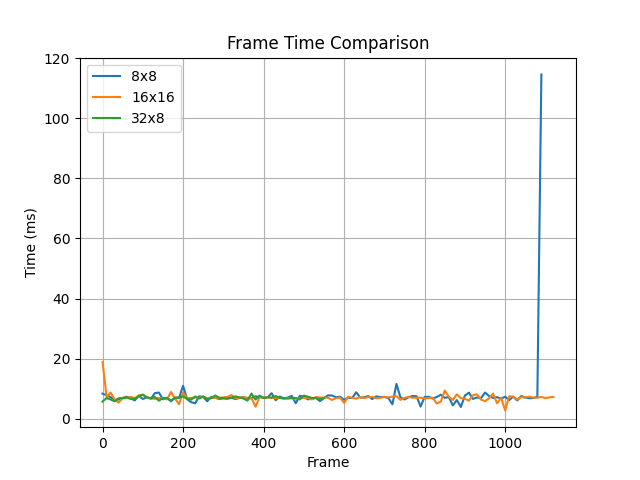
\includegraphics[width=\textwidth]{frame_time_comparison.png}
            \caption{Frame Time Comparison}
            \label{fig:compare_frametime}
        \end{subfigure}
        \caption{Direct comparison of FPS and frame time across all three block size configurations.}
        \label{fig:perf_compare}
    \end{figure}

    \begin{table}[h]
    \centering
    \begin{tabular}{|l|l|l|l|}
    \hline
    \textbf{Block Size} & \textbf{Mean FPS} & \textbf{Mean Frame Time} & \textbf{Key Advantage} \\
    \hline
    $8\times8$   & Lowest  & Highest & Simple baseline; minimal register pressure \\
    $16\times16$ & High    & Low     & 2D spatial locality; better cache use \\
    $32\times8$  & Highest & Lowest  & Warp-aligned coalesced row reads \\
    \hline
    \end{tabular}
    \caption{Qualitative comparison of block size configurations}
    \label{Table:blockcompare}
    \end{table}

    The comparison reveals the trade-offs between block size and layout. The $8\times8$ 
    baseline, while functionally correct, exhibits the highest mean frame time and the 
    lowest sustained FPS due to its limited thread-block occupancy. Both $16\times16$ 
    and $32\times8$ offer 256 threads per block, but their performance differs in 
    practice: the $32\times8$ layout benefits from warp-aligned coalesced memory access 
    along rows, typically yielding lower kernel times, whereas $16\times16$ improves 
    two-dimensional spatial locality and may show advantages when vertical neighbour 
    accesses (diagonal gravity checks) are the bottleneck. The choice of optimal block 
    geometry is therefore workload-dependent and reflects the classic GPU optimisation 
    tension between occupancy, memory coalescing, and register pressure.

	\subsection{Limitations and Future Work}
	\begin{itemize}
		\item \textbf{Single particle type:} Only sand is implemented. Future work could add water 
        (which spreads horizontally) and fire (which rises upward) as additional cell states, 
        each with their own transition rules and colour palettes.
		\item \textbf{CPU-GPU memory transfer bottleneck:} The per-frame \texttt{cudaMemcpy} of 
        the colour buffer is a performance bottleneck. Replacing it with CUDA--OpenGL PBO 
        interoperability would eliminate this transfer entirely.
		\item \textbf{Fixed resolution:} The grid size is hardcoded at 800$\times$600. 
        A future version could support dynamic resizing by reallocating GPU buffers on window resize.
        \item \textbf{No particle persistence / save:} The simulation state is lost when the 
        application closes. Serialising \texttt{d\_gridInput} to disk would allow scenes to be saved and reloaded.
	\end{itemize}

    \begin{table}[h]
    \centering
    \begin{tabular}{|p{4cm}|p{4.5cm}|p{5cm}|}
    \hline
    \textbf{Limitation} & \textbf{Impact} & \textbf{Proposed Future Work} \\
    \hline
    Single particle type & Limited simulation variety & Add water, fire, smoke with distinct rules \\
    \hline
    CPU--GPU memcpy overhead & 1.92 MB transfer every frame & Replace with CUDA--OpenGL PBO interop \\
    \hline
    Fixed 800$\times$600 resolution & Cannot adapt to window resize & Dynamic GPU buffer reallocation \\
    \hline
    No state persistence & Simulation lost on exit & Serialise \texttt{d\_gridInput} to disk \\
    \hline
    \end{tabular}
    \caption{Known limitations and proposed future improvements}
    \label{Table:limitations}
    \end{table}


% ============================================================
%  REFERENCES
% ============================================================
	\newpage
	\addcontentsline{toc}{section}{References}
	\bibliographystyle{IEEEtran}
	\bibliography{mybib}

\end{document}